\newpage

\chapter{Sprint 1: Site Management and Authentication}

\cfoot{\thepage}

\parindent=0.5in
\onehalfspacing

\usepackage{multirow}

\section{Introduction}

Sprint 1, titled "Site Management and Authentication," establishes the foundational elements essential for all subsequent development phases. This sprint focuses on implementing secure user access control with Supabase authentication and basic site information management capabilities required for telecommunications infrastructure operations.

The sprint addresses four high-priority user stories from Chapter 2's product backlog: US-001 (User Authentication), US-002 (User Profile Management), US-003A-C (Site Management CRUD operations), and US-004 (Site Information Access). These stories form the foundation upon which subsequent sprints build equipment monitoring, intervention planning, and analytics capabilities.

Sprint 1 objectives align with the architectural design presented in Chapter 2, implementing the authentication layer through Supabase Auth, establishing the initial database schema with profiles and sites tables, and creating the presentation layer foundation with Next.js and TypeScript. The implementation demonstrates the layered architecture's effectiveness while establishing role-based access control enforced at multiple levels.

\section{Sprint Backlog}

During sprint planning, we defined the tasks required for Sprint 1 implementation. Table 3.1 presents the sprint backlog with user stories, tasks, complexity assessments, and effort estimates in story points.

\begin{table}[H]
\centering
\small
\begin{tabular}{|p{2.5cm}|p{4cm}|p{3.2cm}|p{2.2cm}|p{1.5cm}|}
\hline
\textbf{Functionality} & \textbf{User Story} & \textbf{Tasks} & \textbf{Complexity} & \textbf{Estimate} \\
\hline

\multirow{3}{2.5cm}{Authentication System} & 
\multirow{3}{4cm}{As admin, engineer, technician, and manager, I can authenticate to access the system}
& Supabase Auth integration & Hard & 8 \\
\cline{3-5}
& & Create login interface & Medium & 3 \\
\cline{3-5}
& & Integration and testing & Hard & 5 \\
\hline

\multirow{3}{2.5cm}{User Profile Management} & 
\multirow{3}{4cm}{As any user, I want to manage my profile and change my password}
& Implement profile management & Medium & 3 \\
\cline{3-5}
& & Create profile interface & Easy & 2 \\
\cline{3-5}
& & Integration and testing & Medium & 3 \\
\hline

\multirow{3}{2.5cm}{Create Site (US-003A)} & 
\multirow{3}{4cm}{As admin, engineer, or manager, I can create new telecommunications sites}
& Implement site creation logic & Medium & 4 \\
\cline{3-5}
& & Create site creation modal & Medium & 3 \\
\cline{3-5}
& & Validation and testing & Medium & 3 \\
\hline

\multirow{3}{2.5cm}{Edit Site (US-003B)} & 
\multirow{3}{4cm}{As admin or engineer, I can edit existing site information. As manager, I can edit site status}
& Implement site edit logic & Medium & 3 \\
\cline{3-5}
& & Create site edit modal & Easy & 2 \\
\cline{3-5}
& & Permission testing & Medium & 3 \\
\hline

\multirow{3}{2.5cm}{Delete Site (US-003C)} & 
\multirow{3}{4cm}{As admin, I can delete decommissioned sites from the system}
& Implement site deletion & Easy & 2 \\
\cline{3-5}
& & Create confirmation modal & Easy & 1 \\
\cline{3-5}
& & Referential integrity testing & Medium & 3 \\
\hline

\multirow{3}{2.5cm}{View Sites (US-004)} & 
\multirow{3}{4cm}{As all users, I can view telecommunications site information}
& Implement site list view & Medium & 3 \\
\cline{3-5}
& & Create site detail view & Medium & 3 \\
\cline{3-5}
& & Real-time updates & Hard & 4 \\
\hline

\multirow{3}{2.5cm}{Role-Based Access Control} & 
\multirow{3}{4cm}{As the system, I enforce different access levels based on user roles}
& Implement RLS policies & Hard & 6 \\
\cline{3-5}
& & Configure role permissions & Medium & 3 \\
\cline{3-5}
& & Test all role combinations & Hard & 4 \\
\hline

\end{tabular}
\caption{Sprint 1 Backlog with Task Breakdown}
\label{tab:sprint1_backlog}
\end{table}

The backlog totals 71 story points across seven user stories, aligning with the two-week sprint duration. The Site Management functionality has been split into three distinct user stories (US-003A, US-003B, US-003C) reflecting the different permission levels and operational contexts: site creation available to administrators, engineers, and managers; site editing with differentiated permissions; and site deletion restricted to administrators only. This granular approach enables precise permission management and facilitates sprint planning.

\section{Conceptual Design}

This section presents the conceptual design models guiding Sprint 1 implementation, ensuring alignment between requirements and technical implementation.

\subsection{Class Diagram}

Figure 3.1 presents the class diagram for Sprint 1, focusing on core entities: Supabase authentication, user profiles, and telecommunications sites.

\begin{figure}[H]
    \centering
    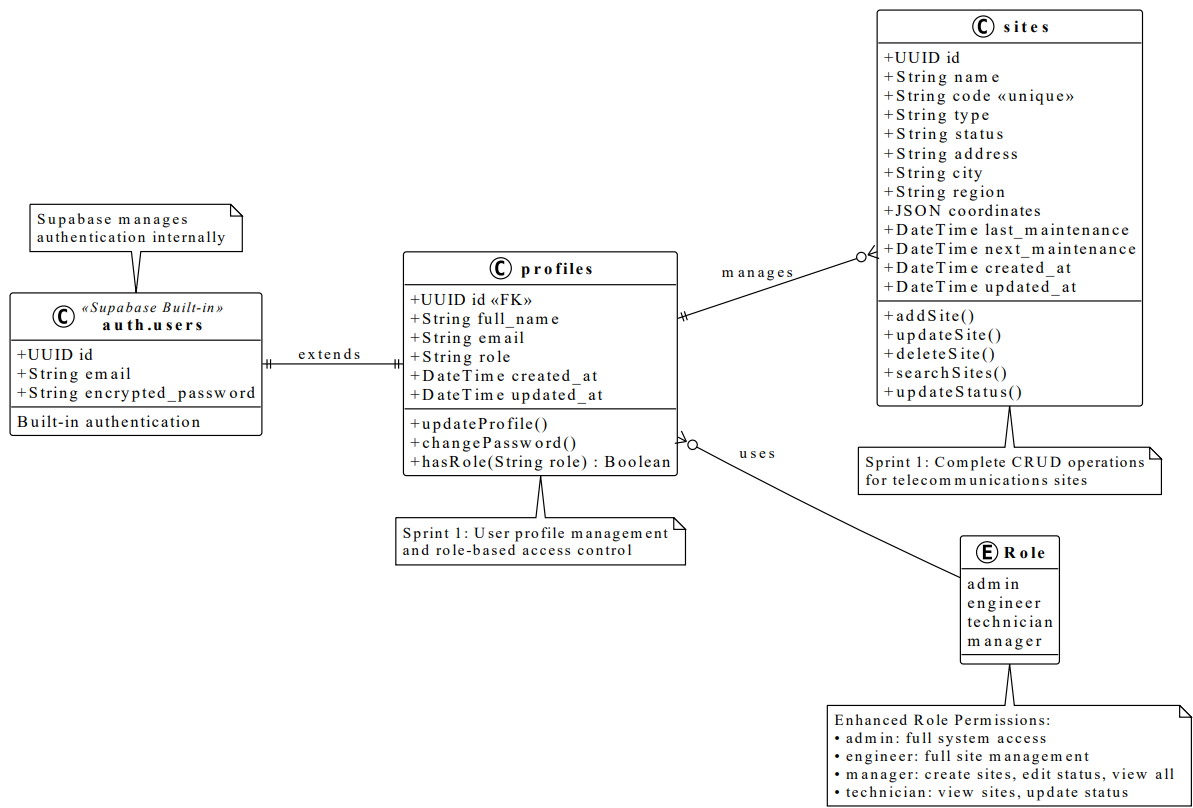
\includegraphics[width=0.95\linewidth]{img/chap_03/class_diagram_sprint1.png}
    \caption{Class Diagram - Authentication and Site Management}
    \label{fig:class_diagram_sprint1}
\end{figure}


The class diagram illustrates relationships between Supabase's built-in authentication system (\texttt{auth.users}), the custom \texttt{profiles} table extending user information with business-specific fields (role, region, full name), and the \texttt{sites} table for telecommunications site management. The \texttt{Role} enumeration defines four distinct user types (admin, engineer, technician, manager) corresponding to the stakeholder roles identified in Chapter 2. Each profile associates with exactly one authentication user, while sites maintain creation and modification audit trails through timestamps and user associations.

\subsection{Use Case Diagram}

Figure 3.2 presents the use case diagram showing actors and their interactions with Sprint 1 functionalities.

\begin{figure}[H]
    \centering
    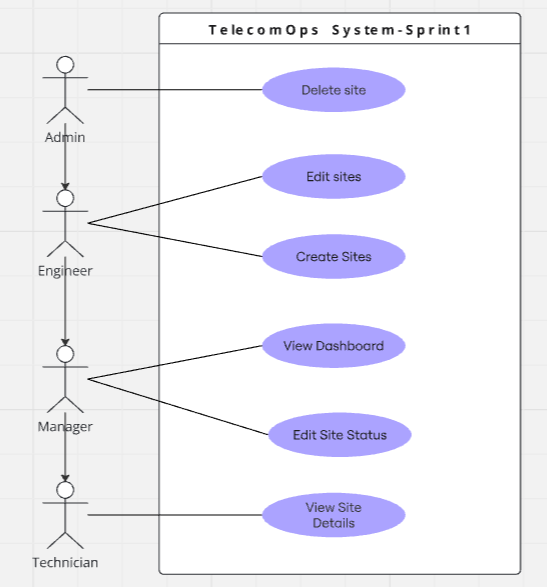
\includegraphics[width=0.85\linewidth]{img/chap_03/use_case_diagram_sprint1.png}
    \caption{Use Case Diagram - Sprint 1 Functionalities}
    \label{fig:use_case_diagram_sprint1}
\end{figure}

The use case diagram shows four primary actors with differentiated permission levels reflecting the stakeholder access matrix from Chapter 2, Table 2.1. Administrator has full system access including user management and site deletion. Network Engineer focuses on technical site management with create, edit, and view operations. Manager has operational oversight with site creation and status editing capabilities for deployment approvals and operational decisions. Field Technician has view access supporting field operations.

\textbf{Use Case Description: Create Site}

Since use cases for creating, editing, and deleting sites share similar processing patterns, we provide detailed information on the "Create Site" use case as representative of the site management functionality. Table 3.2 presents the detailed textual description.

\begin{table}[H]
\centering
\begin{tabular}{|p{3.5cm}|p{8cm}|}
\hline
\textbf{Use Case} & Create Site \\
\hline
\textbf{Primary Actors} & Administrator, Network Engineer, Manager \\
\hline
\textbf{Pre-condition} & User successfully authenticated with appropriate role (admin, engineer, or manager) \\
\hline
\textbf{Post-condition} & Site successfully created in database with unique identifier \\
\hline
\textbf{Main Scenario} & 
1. User accesses site management interface
2. User clicks "Add Site" button displaying creation modal
3. User fills form: name, code, address, coordinates, technology type
4. User submits form
5. System validates fields and checks site code uniqueness
6. System verifies user permissions via Row Level Security
7. System creates site in database
8. System updates site list in real-time
9. System displays success confirmation
\\
\hline
\textbf{Exception Scenarios} & 
E1: Missing required data → Display field-specific error messages
E2: Duplicate site code → Display uniqueness violation error
E3: Insufficient permissions → Display access denied error
E4: Server connection problem → Display connection error with retry option
\\
\hline
\end{tabular}
\caption{Detailed Use Case Description - Create Site}
\label{tab:create_site_usecase}
\end{table}

\section{Sequence Diagrams}

This section presents sequence diagrams detailing the main processes implemented in Sprint 1, illustrating interactions between system components.

\subsection{Authentication Process}

Figure 3.3 illustrates the complete user authentication workflow using Supabase authentication services.

\begin{figure}[H]
    \centering
    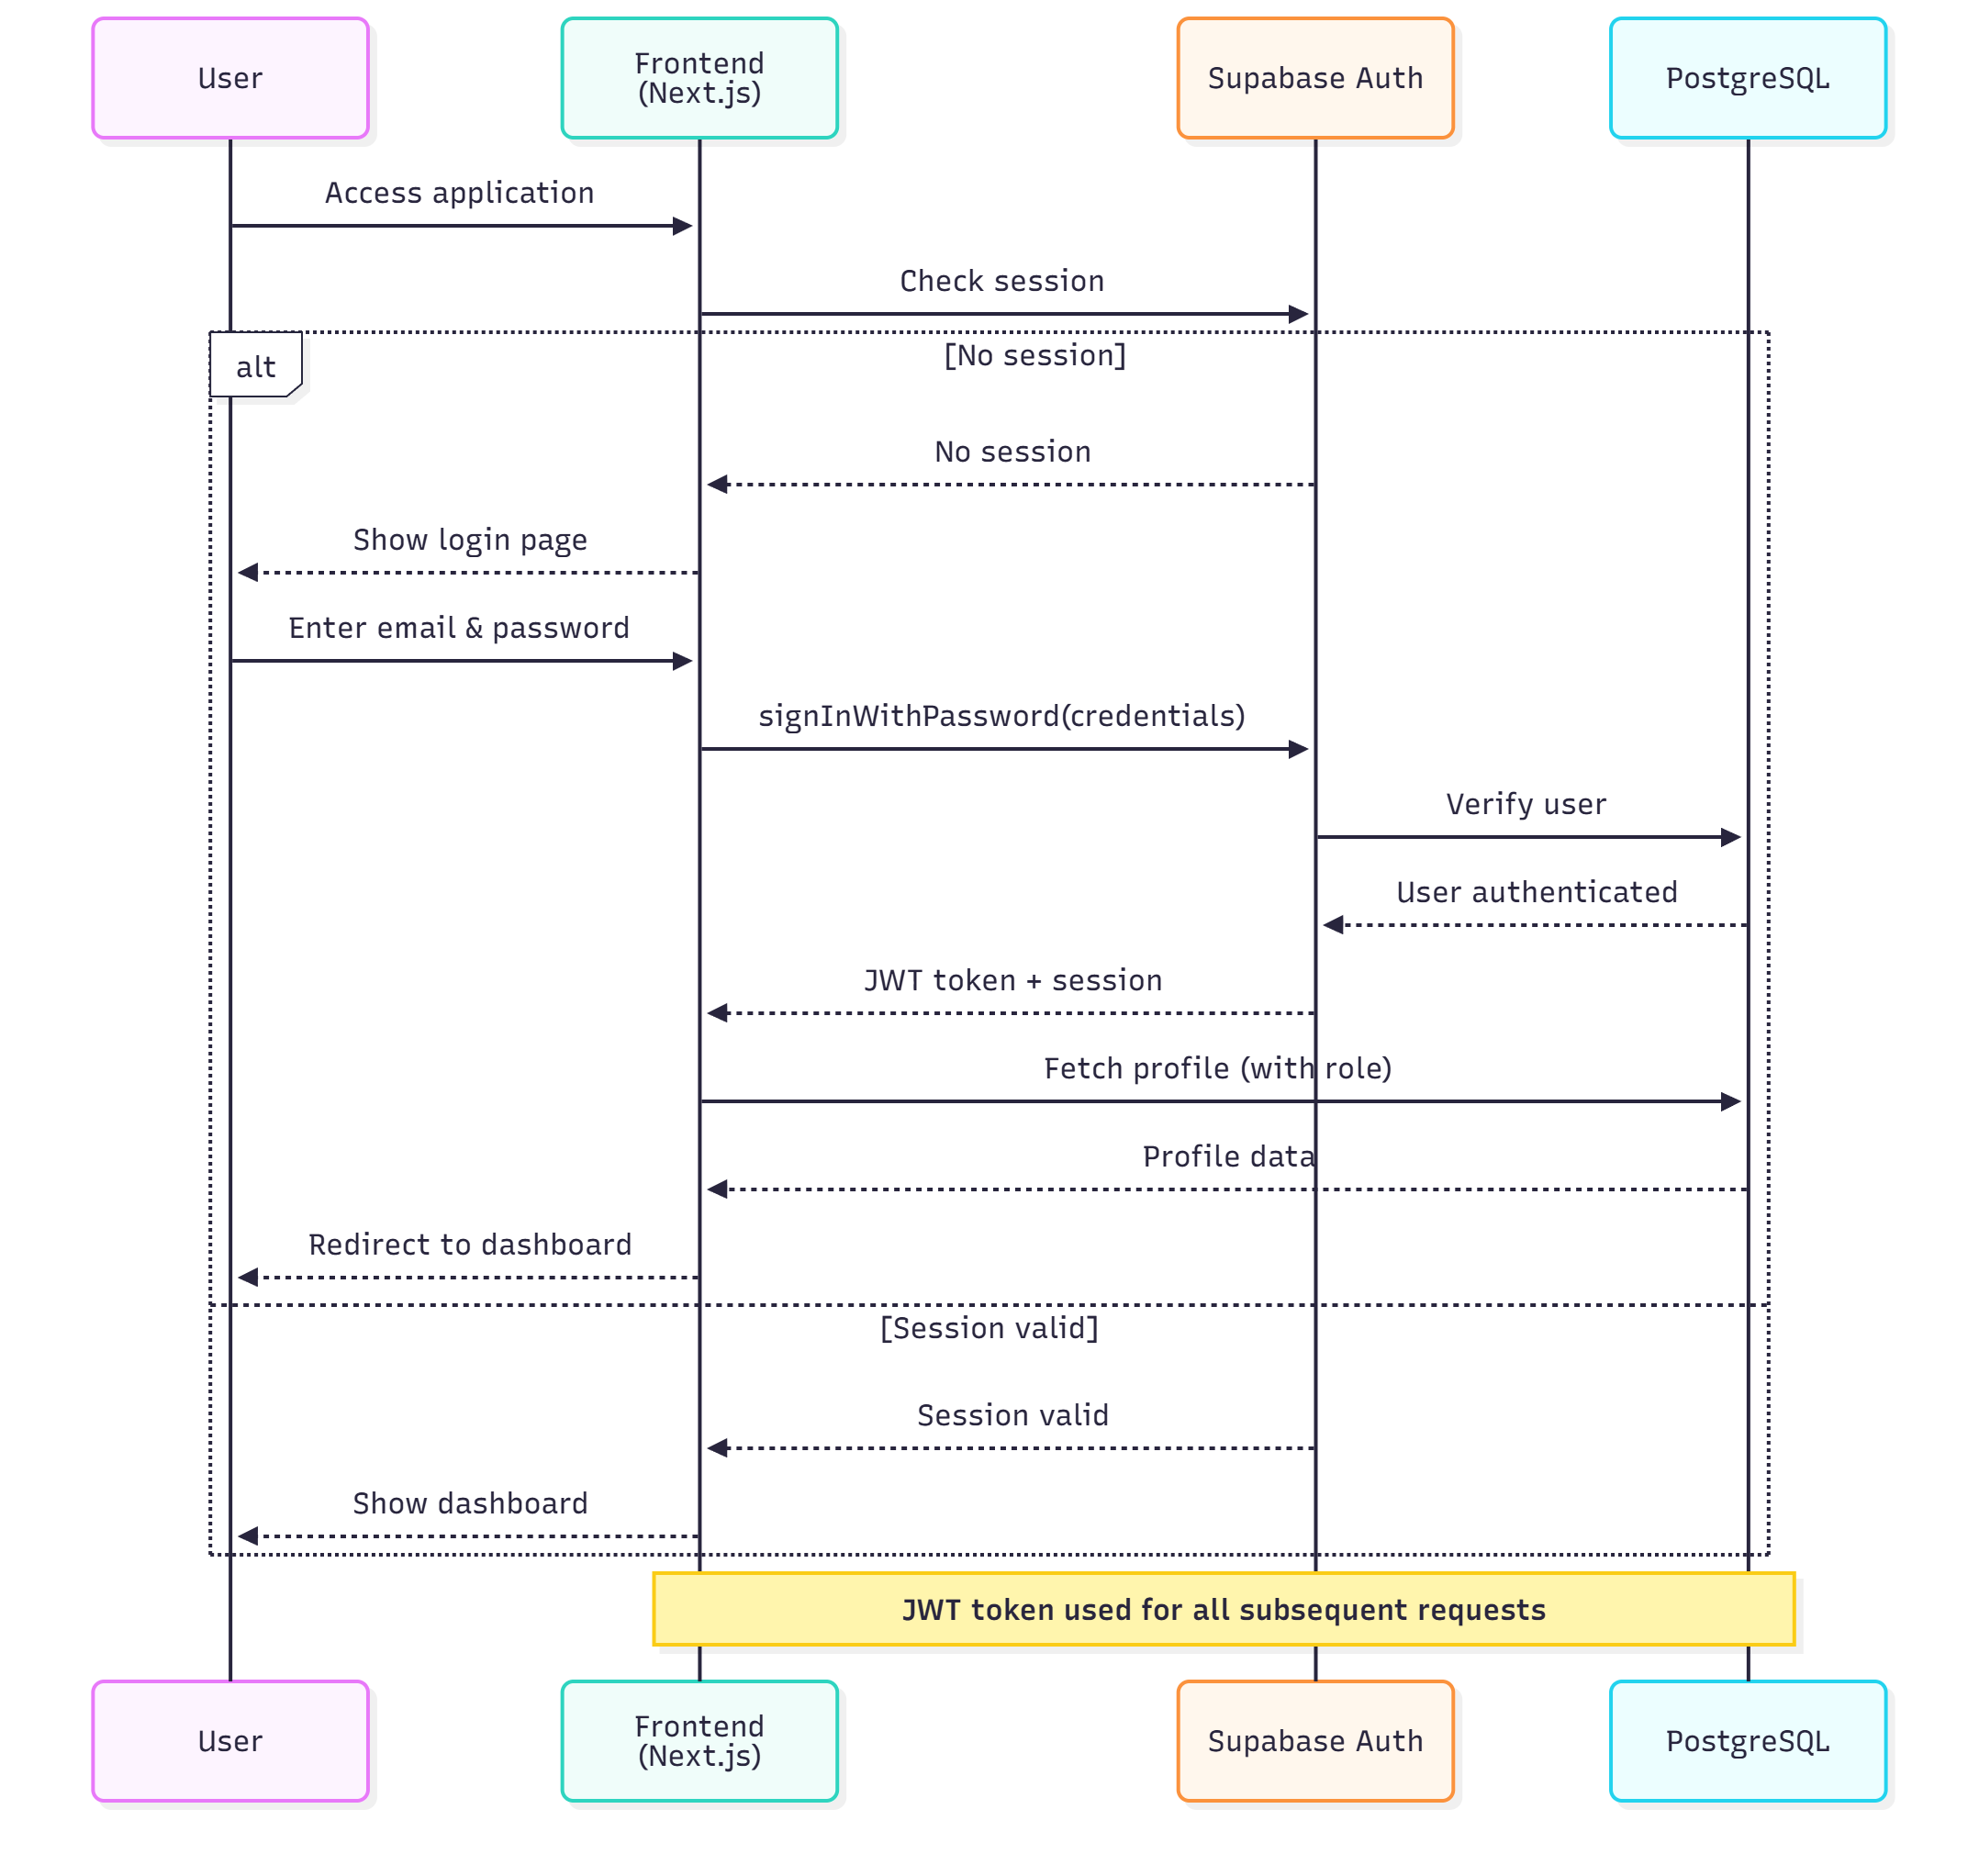
\includegraphics[width=0.95\linewidth]{img/chap_03/sequence_authentication.png}
    \caption{Sequence Diagram - Authentication Process}
    \label{fig:sequence_authentication}
\end{figure}

\textbf{Note on Sequence Diagram:} In proper UML sequence diagram notation, return messages should be represented with dashed lines (dotted lines) rather than solid lines, distinguishing them from request messages. The diagram should show request messages as solid arrows and return messages as dashed arrows to maintain standard UML conventions.

The authentication sequence (Figure 3.3) demonstrates the login process implementing Chapter 2's security architecture. When users access the application, the system checks for existing valid sessions. Without valid sessions, users enter credentials which undergo client-side validation before transmission to Supabase Auth via \texttt{signInWithPassword()}. Supabase verifies credentials against PostgreSQL, generates JWT tokens containing user identification upon success, and returns session information. The frontend fetches user profiles including roles using Row Level Security-protected queries, stores sessions locally, and redirects users to role-appropriate dashboards. Failed authentication displays error messages, while valid existing sessions grant direct dashboard access.

\subsection{Site Creation Process}

Figure 3.4 demonstrates the complete workflow for adding telecommunications sites to the system.

\begin{figure}[H]
    \centering
    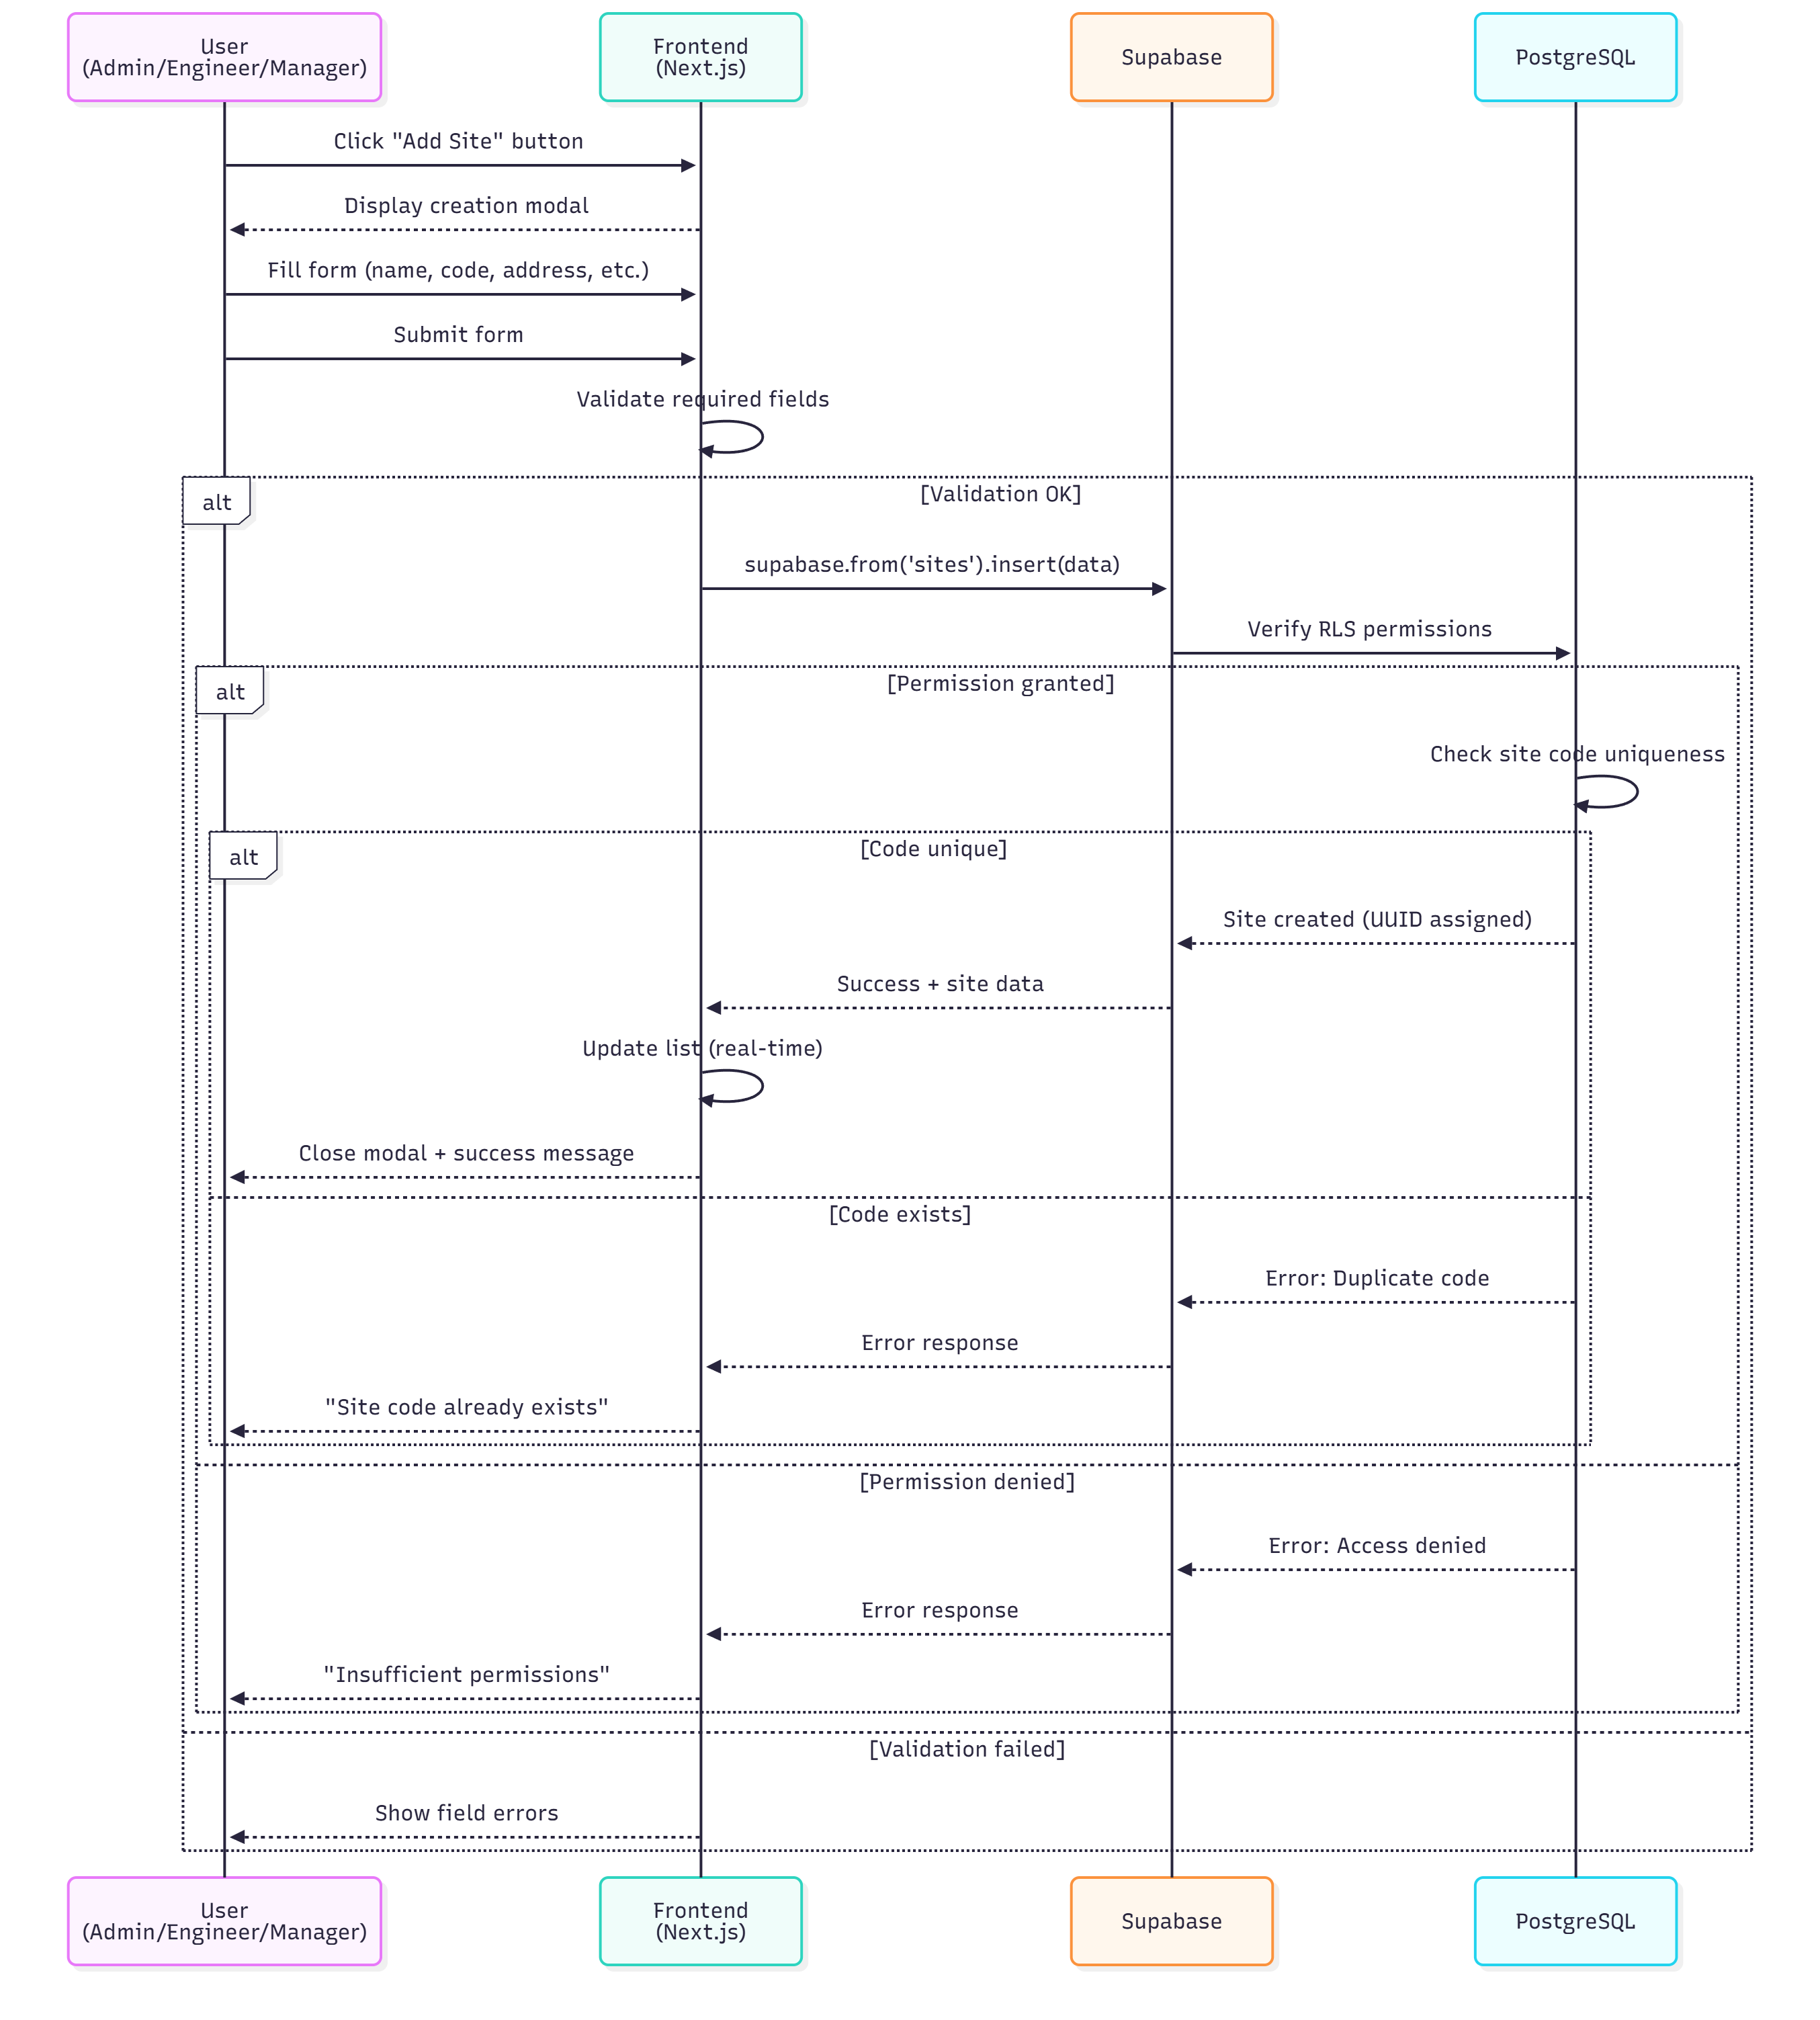
\includegraphics[width=0.95\linewidth]{img/chap_03/sequence_add_site.png}
    \caption{Sequence Diagram - Create Site Process}
    \label{fig:sequence_add_site}
\end{figure}

The site creation sequence (Figure 3.4) shows authorized users (Administrator, Engineer, Manager) accessing the site management interface and clicking "Add Site" to display the creation modal. After completing site details (name, unique code, address, technology type), form submission triggers comprehensive validation checking required fields and code format. Valid requests proceed to Supabase database via \texttt{supabase.from('sites').insert()}. The database performs two critical security checks: Row Level Security policy validation ensuring only authorized roles can create sites, and unique constraint checking preventing duplicate site codes. Successful validation results in site insertion with UUID assignment, real-time list updates via Supabase subscriptions, modal closure, and success confirmation. Constraint violations or validation failures display appropriate error messages guiding corrective action.

\section{Implementation}

This section presents screenshots illustrating the interfaces developed during Sprint 1 implementation, demonstrating the application's user experience design.

\subsection{Authentication Interface}

Figure 3.5 illustrates the authentication interface implementing Supabase's secure authentication system with email and password validation.

\begin{figure}[H]
    \centering
    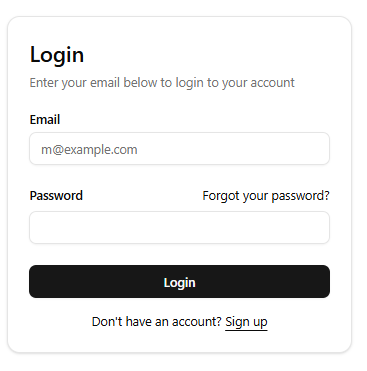
\includegraphics[width=0.7\linewidth]{img/chap_03/login_interface.png}
    \caption{Login Interface with Supabase Authentication}
    \label{fig:login_interface}
\end{figure}

\subsection{Dashboard Interfaces}

Figures 3.6 and 3.7 illustrate the role-based dashboard providing different views based on user roles, with the main dashboard showing key metrics and the sites management interface displaying the comprehensive site list with action buttons.

\begin{figure}[H]
    \centering
    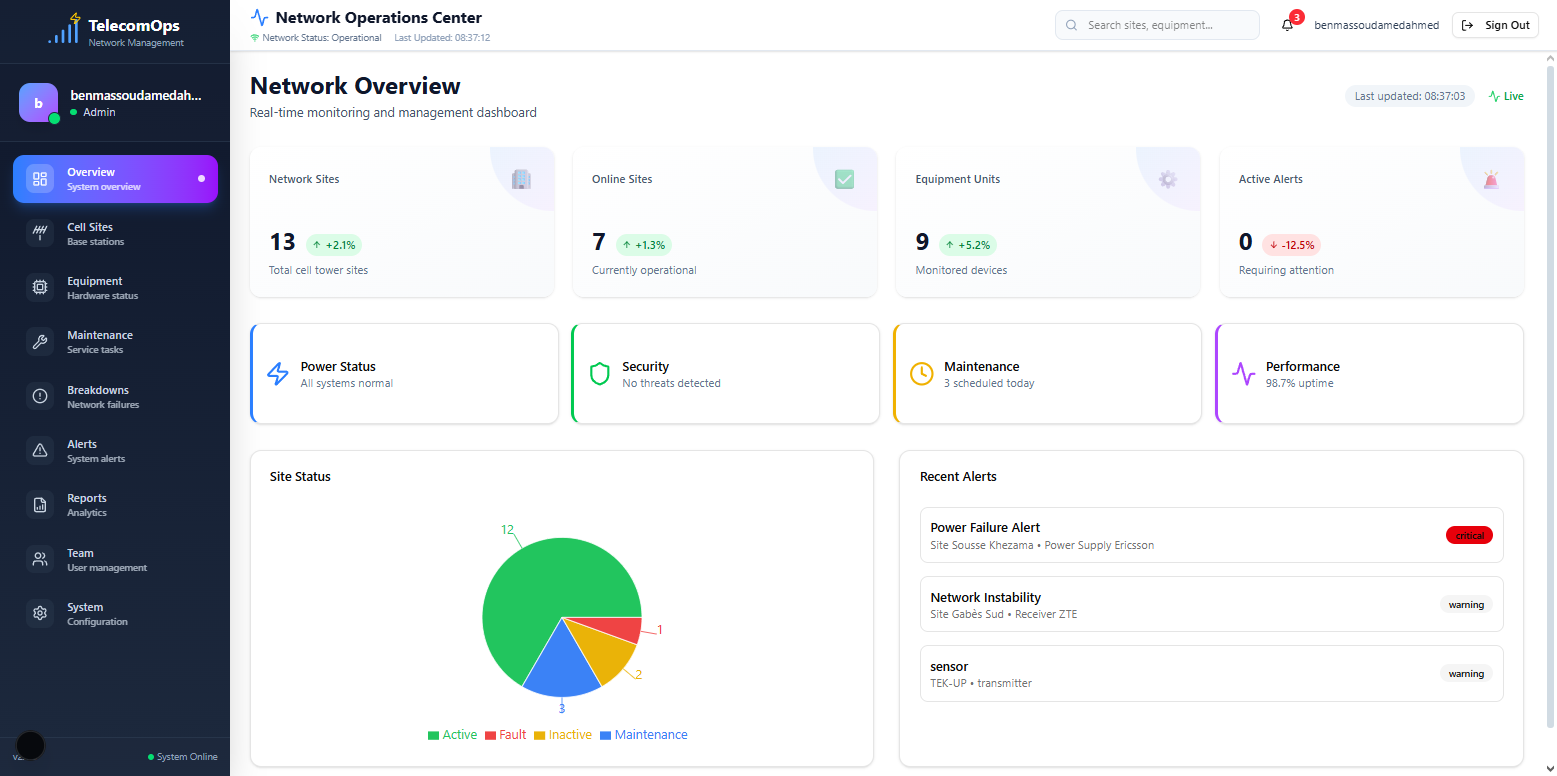
\includegraphics[width=0.9\linewidth]{img/chap_03/dashboard_main.png}
    \caption{Main Dashboard with Role-Based Metrics}
    \label{fig:dashboard_main}
\end{figure}

\begin{figure}[H]
    \centering
    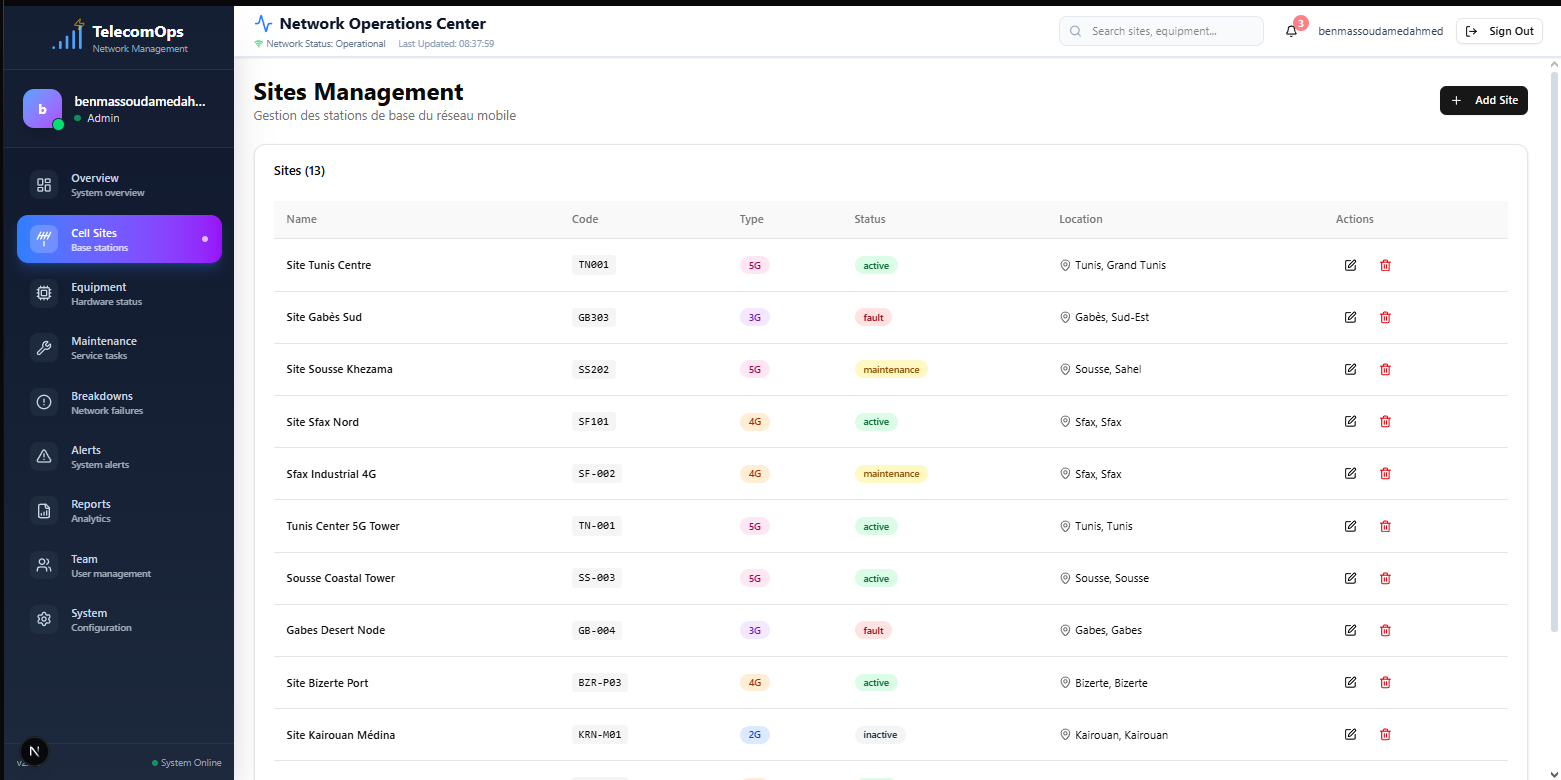
\includegraphics[width=0.9\linewidth]{img/chap_03/sites_list.png}
    \caption{Sites Management Interface with Action Controls}
    \label{fig:sites_list}
\end{figure}

\subsection{Site Management Modals}

Figures 3.8, 3.9, and 3.10 illustrate the site management modals implementing the CRUD operations with appropriate permission checks enforced through Row Level Security.

\begin{figure}[H]
    \centering
    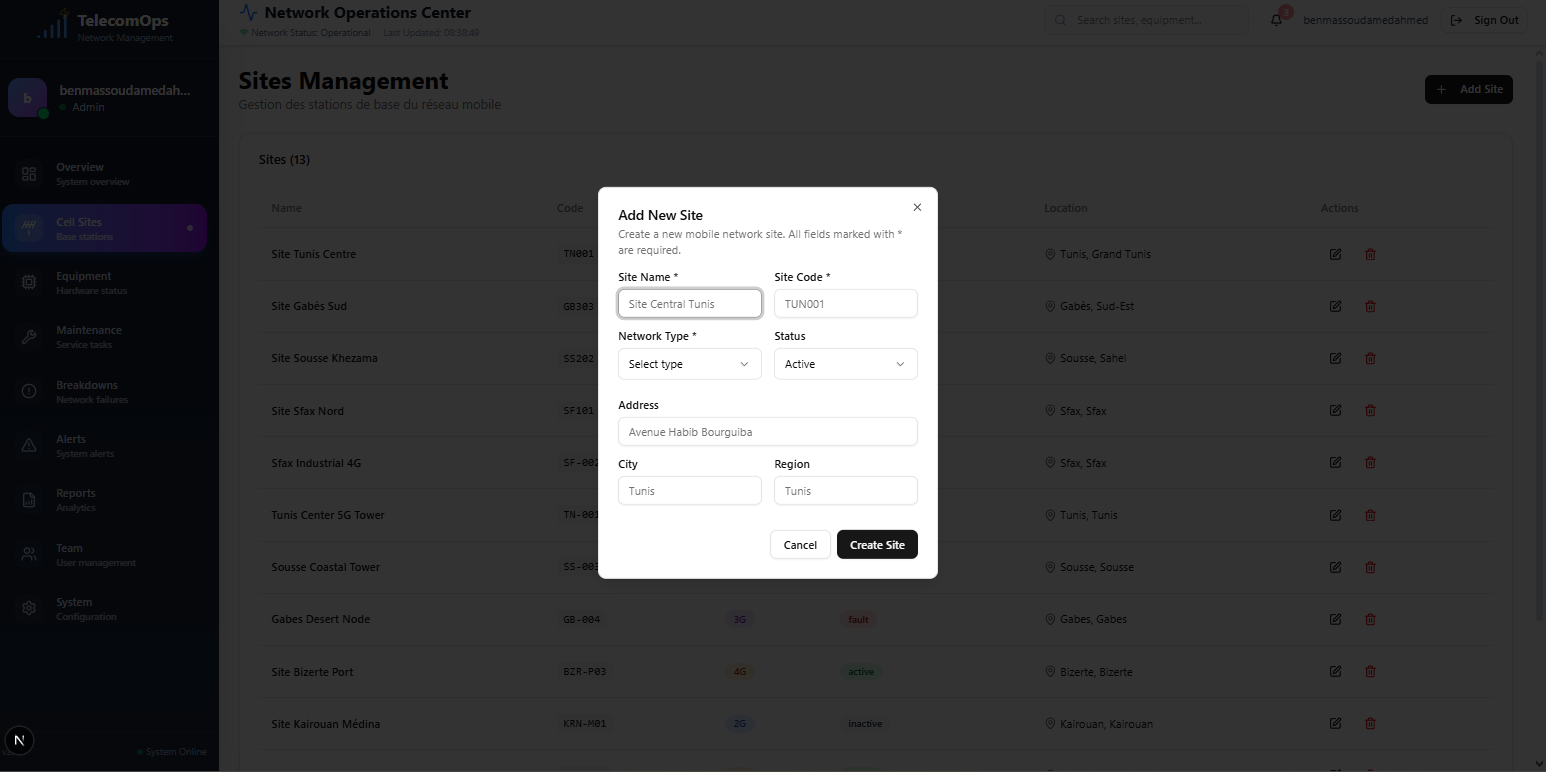
\includegraphics[width=0.85\linewidth]{img/chap_03/create_site_modal.png}
    \caption{Create Site Modal with Form Validation}
    \label{fig:add_site_modal}
\end{figure}

\begin{figure}[H]
    \centering
    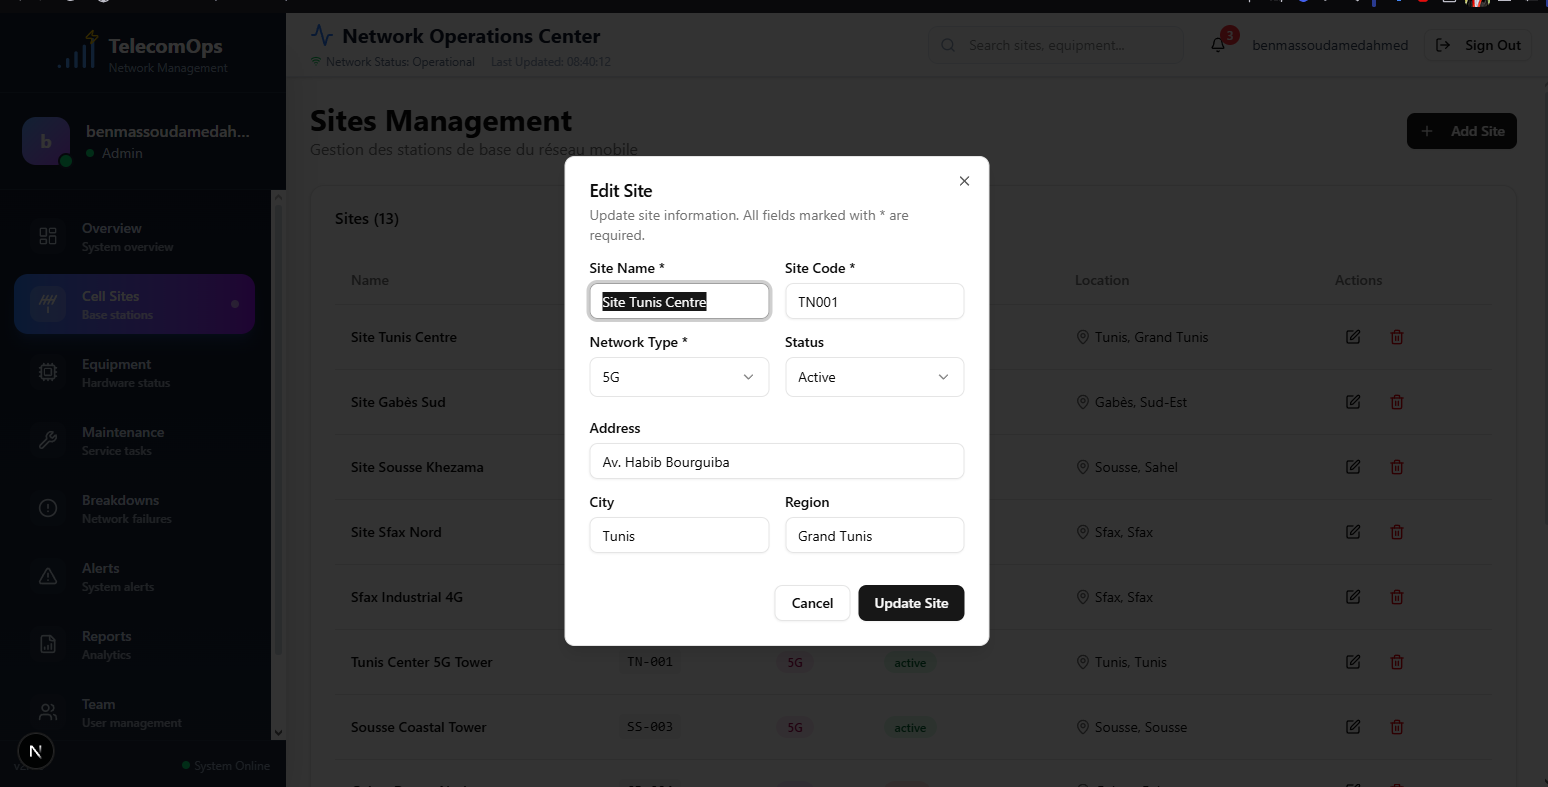
\includegraphics[width=0.85\linewidth]{img/chap_03/edit_site_modal.png}
    \caption{Edit Site Modal with Pre-populated Data}
    \label{fig:edit_site_modal}
\end{figure}

\begin{figure}[H]
    \centering
    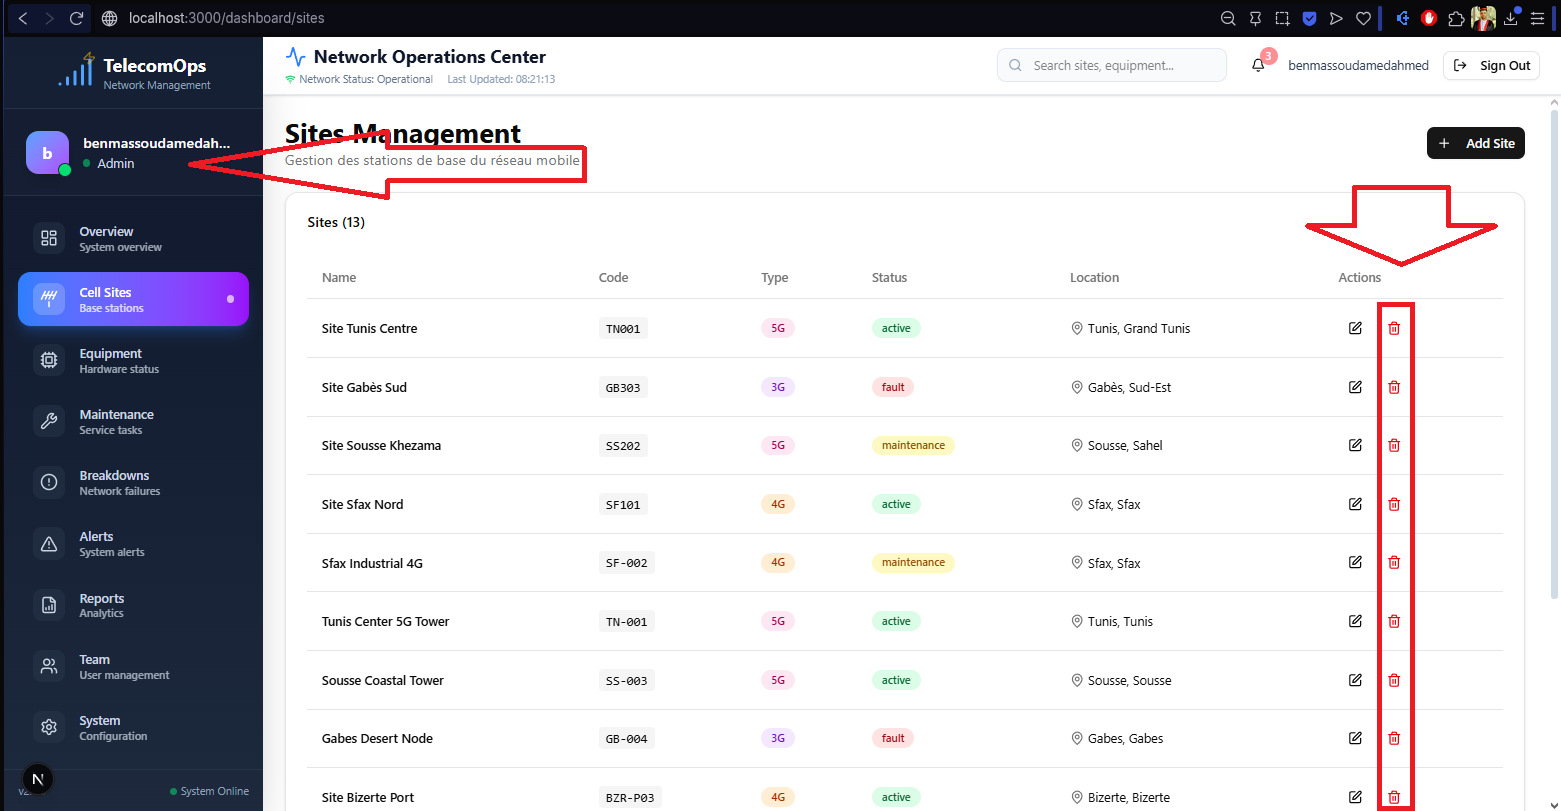
\includegraphics[width=0.85\linewidth]{img/chap_03/delete_site_modal.png}
    \caption{Delete Site Confirmation Modal}
    \label{fig:delete_site_modal}
\end{figure}

\subsection{User Profile Management}

Figure 3.11 illustrates the user profile management interface where users update personal information and change passwords securely.

\begin{figure}[H]
    \centering
    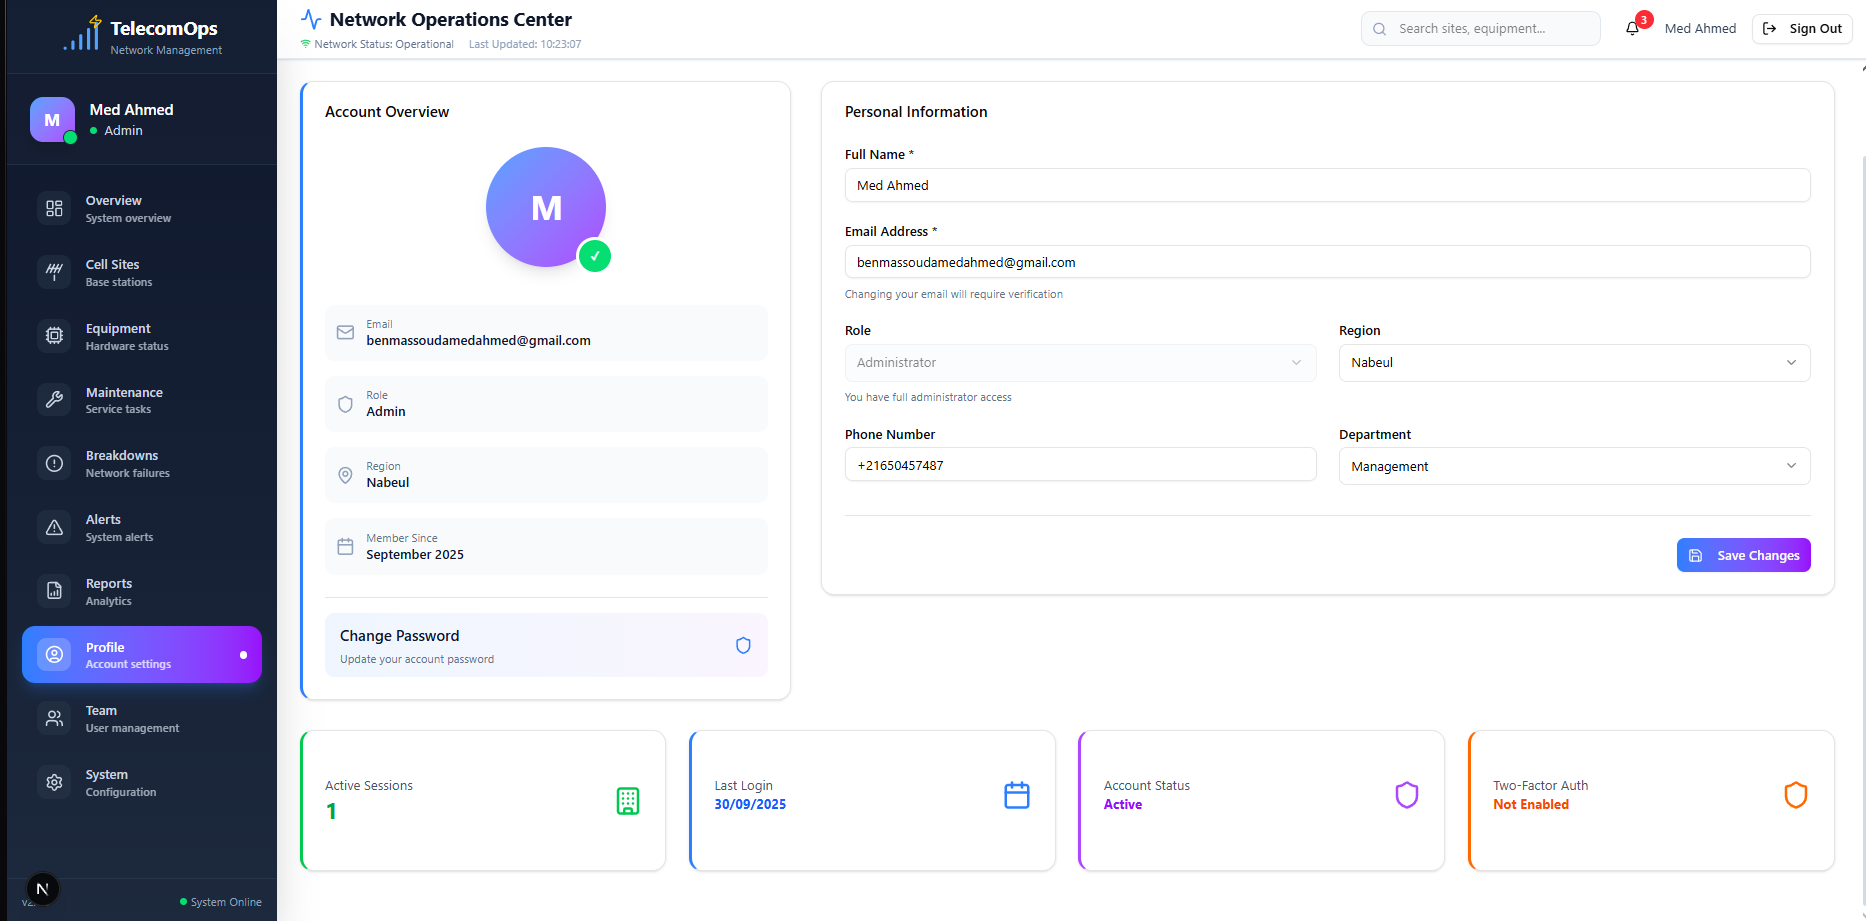
\includegraphics[width=0.85\linewidth]{img/chap_03/profile_management.png}
    \caption{User Profile Management Interface}
    \label{fig:profile_management}
\end{figure}

\section{Technical Challenges and Solutions}

Sprint 1 implementation encountered several technical challenges requiring careful analysis and innovative solutions.

\subsection{Row Level Security Configuration}

Implementing comprehensive Row Level Security policies presented significant complexity. Initial configurations caused permission errors preventing legitimate operations. Resolution involved developing granular RLS policies distinguishing between user roles while maintaining security. Policies now properly enforce that administrators, engineers, and managers can create and edit sites, while all authenticated users view site information. The enhanced Manager role required specific policies granting create and update permissions while restricting delete operations to administrators only.

\subsection{Real-time Data Synchronization}

Ensuring data consistency across multiple users accessing sites simultaneously required implementing Supabase's real-time subscriptions. When one user creates or updates sites, all connected users see changes immediately without page refresh. This was achieved through WebSocket connections managed by Supabase's real-time engine, implementing the real-time capabilities specified in Chapter 2's application layer architecture.

\subsection{Session Management and Security}

Implementing secure session management with automatic timeout required careful JWT token handling. The solution implements 30-minute inactivity timeout with automatic token refresh, secure token storage in memory rather than localStorage preventing XSS attacks, and session validation on each protected route access. This addresses NFR-004 authentication security requirements from Chapter 2.

\section{Testing and Validation}

Sprint 1 underwent comprehensive testing ensuring reliability, security, and proper role-based access control as specified in Chapter 2's success criteria.

\subsection{Authentication Security Testing}

Testing validated authentication bypass prevention, session management, and password security. All tests confirmed Supabase authentication properly protects against SQL injection, cross-site scripting, and brute force attacks. Failed login attempts trigger appropriate delays, and account lockout activates after five consecutive failures.

\subsection{Role-Based Access Testing}

Each user role was tested verifying appropriate access levels. Table 3.3 summarizes role testing results.

\begin{table}[H]
\centering
\small
\begin{tabular}{|l|c|c|c|c|}
\hline
\textbf{Operation} & \textbf{Admin} & \textbf{Engineer} & \textbf{Technician} & \textbf{Manager} \\
\hline
View Sites & Allowed & Allowed & Allowed & Allowed \\
\hline
Create Site & Allowed & Allowed & Denied & Allowed \\
\hline
Edit Site & Allowed & Allowed & Denied & Allowed (Status Only) \\
\hline
Delete Site & Allowed & Denied & Denied & Denied \\
\hline
Manage Users & Allowed & Denied & Denied & Denied \\
\hline
\end{tabular}
\caption{Role-Based Access Testing Results}
\label{tab:role_testing}
\end{table}

All unauthorized operations were properly blocked by Row Level Security policies, confirming the security architecture's effectiveness.

\subsection{Site Management Functional Testing}

Complete CRUD operations were validated: site creation with unique code enforcement preventing duplicates, site editing with proper field validation ensuring data integrity, site deletion restricted to administrators with referential integrity checking, and real-time list updates across multiple user sessions confirming WebSocket functionality. All tests passed successfully, meeting the success criteria defined in Chapter 2, Section 2.5.2.

\subsection{Performance Testing}

Performance testing validated NFR-001 requirements from Chapter 2. Page load times averaged 2.1 seconds (target: under 3 seconds), API response times averaged 280ms (target: under 500ms), and real-time updates propagated within 1.5 seconds (target: within 2 seconds). All performance metrics exceeded established targets.

\section{Sprint Review and Retrospective}

Sprint 1 review with stakeholders confirmed successful delivery of all committed user stories. Stakeholders approved the authentication system's security implementation, site management interface's usability, and role-based access control's accurate reflection of organizational structure. User acceptance testing across all four user roles validated the implementation meets operational requirements.

The sprint retrospective identified several positive outcomes: Supabase integration accelerated development by providing authentication infrastructure without custom backend development; TypeScript type safety prevented numerous potential runtime errors during development; and Next.js server-side rendering provided excellent initial page load performance. Areas for improvement include earlier stakeholder involvement in interface design and more comprehensive integration testing earlier in the sprint.

\section{Conclusion}

Sprint 1 successfully established the foundational authentication infrastructure and site management capabilities essential for TelecomOps. The implementation delivered secure user authentication using Supabase Auth, comprehensive site management functionality with CRUD operations split into three distinct user stories (US-003A, US-003B, US-003C) for precise permission management, role-based access control enforced through Row Level Security, and user profile management with password change capabilities.

The sprint addressed all high-priority user stories from Chapter 2's product backlog, implementing the authentication and presentation layers specified in the system architecture. The enhanced Manager role provides appropriate operational oversight capabilities while maintaining security boundaries, reflecting the stakeholder analysis from Chapter 2.

Quality metrics exceeded established targets with successful user acceptance testing across all user roles, performance metrics surpassing NFR-001 requirements, and comprehensive security validation confirming the multi-layer security architecture's effectiveness. The implementation demonstrates effective integration of Next.js, TypeScript, and Supabase while addressing real-world telecommunications operational requirements.

Sprint 1 establishes a robust foundation for subsequent development. The authentication infrastructure enables all future features requiring user identification and authorization. The site management foundation provides the core entity upon which equipment inventory, interventions, and monitoring features will build in subsequent sprints.

The next chapter presents Sprint 2, titled "Equipment Monitoring and Inventory Management," which extends the site management foundation with comprehensive equipment tracking, lifecycle management, and maintenance scheduling capabilities, addressing user stories US-005A-C, US-006, and US-016A-B from the product backlog.